\newcommand*{\crt}{\mathrm C}
\newcommand*{\tri}{_\mathrm{tr}}


\chapter{相与相变}
\label{chap:phase}

\begin{definition}
	{相}{phase}
	物质的相(phase)是指其化学组份和物理性质在空间上均匀的形态。
	比如:
	\begin{itemize}
		\item 固相(solid phase):分子在晶格上有序排列,具有长程有序性;
		\item 液相(liquid phase):分子在空间上无序排列,具有短程有序性;
		\item 气相(gas phase):分子在空间上完全无序,几乎没有相互作用。
	\end{itemize}
\end{definition}

\begin{remark}
	一个相可以是单组份,例如水,也可以由彼此不发生化学反应的多组份构成,例如溶液。
\end{remark}

% 在一定条件下,不同的相可以共存。不同相之间的转变称为相变。相变发生在外部条件发生变化时,即强度量变化时。相变是竞争的结果。微观上有各种不同的相互作用。不同的相互作用可能会导致不同类型的相变。系统中两个能量尺度间的关系在强度量变化时发生变化。这种关系变化到一定程度后,系统出现新的相。例如,微观上原子分子的相互作用和热运动的相互竞争。控制这两个因素的参量可以是温度(也可以是压强)。在低温时,物质倾向于形成有长程关联的有序结构,这是分子间相互作用的结果。在高温,熵的作用占优势。这种竞争导致相变。相变可以发生在某一温度处,即相变温度,该温度将低温相和高温相隔开。在降温过程中,当微观上相互作用的能量与热运动能量可比拟时,相变发生,出现新的秩序。

\section{化学势}
\label{sec:chemical potential}

我们在前文没有讨论开放系统中的平衡问题。
与封闭系统不同,开放系统的摩尔数$n$不是恒定不变的,由此需要引入新的强度量。

\begin{definition}
	{化学势}{chemical potential}
	在确定的温度$T$和压强$p$下,系统的化学势是Gibbs自由能对摩尔数的偏导数:
	\begin{equation}
		\mu=\pu[p,V]Gn.
	\end{equation}
\end{definition}

\begin{corollary}
	利用Euler公式可得$G=n\mu$,摩尔Gibbs自由能$g=\mu$就是化学势。
\end{corollary}

\begin{corollary}
	内能的微分式、Euler方程和Gibbs-Duhem关系分别为
	\begin{subequations}
		\begin{gather}
			\d U=T\d S-p\d V+\mu\d n,\\
			U=TS-pV+\mu n,\\
			S\d T-V\d p+n\d\mu=0.
		\end{gather}
	\end{subequations}
	化学势的引入也带来了更多的Maxwell关系。
\end{corollary}

\begin{example}
	{理想气体的化学势}{}
	由$\mu=G/n$可得
	\begin{equation}
		\mu=\mu_0\frac T{T_0}-RT\ln\biggfkh{\biggkh{\frac T{T_0}}^{c+1}\frac{p_0}p}.
	\end{equation}
\end{example}

\iffalse
由Gibbs自由能给出Maxwell关系
\begin{align*}
	\pw GTN=\pw GNT & \implies\kh{\pv\mu{T}}_N=-\kh{\pv SN}_T=-s, \\
	\pw GPN=\pw GNP & \implies\kh{\pv\mu{P}}_N=\kh{\pv VN}_P=v.
\end{align*}

\begin{example}
	{理想气体的化学势}{}
	前面已经给过,单原子理想气体的熵
	\[
		S=\kB\NA N\ln\fkh{\kh{\frac{4\pi m}{3h^2}}^{3/2}\kh{\frac e\NA}^{5/2}U^{3/2}VN^{-5/2}}.
	\]
	故
	\begin{align*}
		\mu=-T\pv SN
		%&=-\kB\NA T\ln\fkh{\kh{\frac{4\pi mU}{3h^2}}^{3/2}\kh{\frac e{\NA N}}^{5/2}V}+\frac52\kB\NA T\\
		%&=-\kB\NA T\ln\fkh{\kh{\frac{4\pi mU}{3h^2}}^{3/2}\kh{\frac 1{\NA N}}^{5/2}V}\\
		=-\kB\NA T\ln\fkh{\kh{\frac{2\pi m\kB T}{h^2}}^{3/2}\kh{\frac V{\NA N}}}.
	\end{align*}
	注意到热运动的de Broglie波长
	\[
		\lambda=\frac h{\sqrt{2\pi m\kB T}}.
	\]
	且分子数密度$n:=\NA N/V$,因此
	\begin{equation}
		\mu=RT\ln(n\lambda^3).
	\end{equation}
\end{example}
\fi

\section{相变}
\label{sec:phase transition}

考虑单组份的孤立系统中共存的两个相(记为$\phI,\phII$),有
\begin{align*}
	U_\phI+U_\phII&=U\tot,\\
	V_\phI+V_\phII&=V\tot,\\
	n_\phI+n_\phII&=n\tot.
\end{align*}
平衡条件要求
\[
	\d S=\d S_\phI+\d S_\phII
	=\biggkh{\frac1{T_\phI}-\frac1{T_\phII}}\d U_\phI
	+\biggkh{\frac{p_\phI}{T_\phI}-\frac{p_\phII}{T_\phII}}\d V_\phI
	-\biggkh{\frac{\mu_\phI}{T_\phI}-\frac{\mu_\phII}{T_\phII}}\d n_\phI
	=0.
\]
可得
\begin{subequations}
	\begin{align}
		T_\phI&=T_\phII,\\
		p_\phI&=p_\phII,\\
		\mu_\phI&=\mu_\phII.
	\end{align}
\end{subequations}
因此平衡时两相的温度、压强和化学势都是相同的,这分别对应热平衡、力学平衡和相平衡。
当$\mu_\phI\neq\mu_\phII$时,$n_\phI,n_\phII$会对应增减直到达到新的平衡,
相当于一部分物质从一个相变到了另一个相,称为相变(phase transition)。
也就是说,化学势决定了相变。

考虑相变的方向,物体最常见的三种相——固、液、气——之间的转变共有6种。每种都有对应的名称,如\figref{fig:phase transition} 所示。
这些相变的过程在日常生活中也是常见的。

\begin{center}
	\includegraphics[page=6]{figures/tikz/layouts.pdf}
	\captionof{figure}{固液气相变}
	\label{fig:phase transition}
\end{center}

\subsection{相图}
\label{ssec:phase graph}

表示相平衡系统的组成与一些参数(如$p,T,V,\mu$)之间关系的图叫相图。
\begin{center}
	\includegraphics[page=8]{figures/tikz/coordinates.pdf}
	\captionof{figure}{水的$p\vs T\vs V$相图(示意图)}
	\label{fig:H2O phase P-T-V}
	% \footnote{这张图花了我老长时间了。}
\end{center}

\paragraph{$p\vs T$相图}

将\figref{fig:H2O phase P-T-V} 投影到$p\vs T$坐标上,如\figref{fig:H2O phase P-T} 所示,
固液气三相分别占据了不同的区域,区域的边界线上两个相共存。
相共存线的斜率,也就是熔点、沸点或升华点随压强的变化符合Clapeyron方程。

\begin{theorem}
	{Clapeyron方程}{Clapeyron equation}
	相共存曲线下$\mu_\phI=\mu_\phII$,
	由$\d\mu=-s\d T+v\d p$可得
	\[
		(s_\phI-s_\phII)\d T=(v_\phI-v_\phII)\d p\implies\dv Tp=\frac{v_\phI-v_\phII}{s_\phI-s_\phII}.
	\]
	定义单位摩尔系统$\phI\to\phII$吸收的相变潜热(latent heat)为$\ell:=T(s_\phI-s_\phII)$,则有
	\begin{equation}
		\dv Tp=\frac{T(v_\phI-v_\phII)}\ell.
	\end{equation}
\end{theorem}

\begin{corollary}
	一般的气 - 液相变$v_\phg\gg v_\phl$,若气相符合理想气体,并且近似认为相变潜热与温度无关(这个近似是十分粗糙的),可得 
	\[
		\dv Tp\approx\frac{Tv_\phg}\ell=\frac{RT^2}{\ell p}\implies p=p_0\exp\biggfkh{\frac\ell{R}\biggkh{\frac1{T_0}-\frac1T}}.
	\]
	
\end{corollary}

\begin{remark}
	水凝固存在反常膨胀,$v_\phl<v_\phs$,$\d T/\d p<0$。
	% 在Celsius温标下,$\SI{1}{atm}=\SI{101325}{Pa}$下水的凝固点和沸点分别为$\SI{0}{\degreeCelsius}$和$\SI{100}{\degreeCelsius}$。
\end{remark}

\begin{center}
	\includegraphics[page=9]{figures/tikz/coordinates.pdf}
	\captionof{figure}{水的$p\vs T$相图(示意图)}
	\label{fig:H2O phase P-T}
\end{center}

特别地,随着温度的升高,气液共存线会存在一个终点,称为临界点(critical point)。
当$T>T_\crt$时,气液两相将不可分辨,或者说只有气相。
这将在\secref{ssec:liquid-gas phase transition}讨论。
水的临界点$T_\crt=\SI{647.1}{K},p_\crt=\SI{22.064}{MPa}$。

三条相共存线会交于一点,该点代表固液气三相共存,称为三相点(triple point)。
在Kelvin温标下,水的三相点$T\tri=\SI{273.16}{K},p\tri=\SI{611.73}{Pa}$。

\paragraph{$p\vs V$相图}

投影到$p\vs V$\figref{fig:H2O phase P-V} 上,画出等温线。
当$T>T_\crt$时,全为气相区;
当$T<T_\crt$时,会存在气液共存区,对应$p\vs T$图上的气液共存线,因此$p,T$是一一对应的,即等温线在气液共存区内是一条垂直于$p$轴的直线。

\begin{example}
	{杠杆原理}{}
	气液共存区中的等温线代表确定的$p,T$下可以有不同的体积,这与气液两相的摩尔比有关。
	等温线在气液共存区的两端表示全为液相或气相,对应的摩尔体积为$v_\phl,v_\phg$;
	而在共存区内,若液、气相所占的摩尔比分别为$x_\phl,x_\phg$,则其摩尔体积满足杠杆原理:
	\[
		v=v_\phl x_\phl+v_\phg x_\phg\iff x_\phg=\frac{v-v_\phl}{v_\phg-v_\phl}.
	\]
\end{example}

\begin{center}
	\includegraphics[page=11]{figures/tikz/coordinates.pdf}
	\captionof{figure}{$p\vs V$相图(示意图)和等温线}
	\label{fig:H2O phase P-V}
\end{center}

当$T=T_\crt$时,作为$T\to T_\crt$的极限,等温线在临界点C处应有$(\p p/\p V)_T=0$,
此外,平衡态的稳定性要求:
\[
	\pv[2]Gp=\pu[T]Vp\leq 0,\implies\pu[T]pV\leq 0.
\]
因此临界点C只能是等温线上的一个拐点,即
\begin{equation}
	\label{eq:critical point}
	\pu[T]pV=0,\quad\biggkh{\pv[2]pV}_T=0.
\end{equation}

\begin{example}
	{van der Waals气体的约化变量}{vdW critical}
	理想气体不存在液化,考虑van der Waals气体。
	% 对于临界温度$T_\crt$
	% \begin{align*}
	% 	\pv pv&=-\frac{RT}{(v-b)^2}+\frac{2a}{v^3}=0, \\
	% 	\pv[2]pv&=\frac{2RT}{(v-b)^3}-\frac{6a}{v^4}=0.
	% \end{align*}
	代入临界点的拐点条件,解得
	\begin{subequations}
		\label{eq:vdW critical}
		\begin{align}
			v_\crt&=3b,\\
			T_\crt&=\frac{8}{27}\frac{a}{Rb},\\
			p_\crt&=\frac{RT_\crt}{v_\crt-b}-\frac a{v_\crt}=\frac1{27}\frac a{b^2}.
		\end{align}
	\end{subequations}
	可以定义约化变量$\tilde T:=T/T_\crt$等,可得状态方程:
	\begin{equation}
		\tilde p=\frac{8\tilde T}{3\tilde v-1}-\frac3{\tilde v^2}.
	\end{equation}
\end{example}

\paragraph{$T\vs V$相图}

投影到$T\vs V$图上与$p\vs V$图类似。
% 只有$p<p_\crt$时才会有气液共存区,共存区的等压线垂直于$T$轴(对应沸点)。

\subsection{气液相变}
\label{ssec:liquid-gas phase transition}

考虑$G\vs p\vs T$相图,每个相的Gibbs自由能都是$p,T$的连续函数,只有Gibbs自由能最低的那个相可以稳定存在,而相等的两相Gibbs自由能确定了相的边界。在边界处,Gibbs自由能仍然是连续的,但其导数就不一定连续了。形成的面就像一张有折痕的纸,如\figref{fig:phase G-p-T} 所示。

\begin{center}
	\includegraphics[page=13]{figures/tikz/coordinates.pdf}
	\captionof{figure}{$G\vs p\vs T$相图}
	\label{fig:phase G-p-T}
\end{center}

\begin{definition}
	{一级相变和连续相变}{}
	至少有一个Gibbs自由能的一阶导数不连续的相变称为一级相变,否则称为连续相变。
\end{definition}

\begin{corollary}
	连续相变的摩尔熵$s=-(\p g/\p T)_p$是连续的,因此没有潜热。
\end{corollary}

\iffalse
\begin{center}
	\begin{tikzpicture}
		\coor33Tg;
		\draw[dashed](1.5,0)--(1.5,1.5);
		\draw[thick](.5,2)--(1.5,1.5)node[midway,above]{$\phl$}--(2.5,.5)node[midway,above]{$\phg$};
	\end{tikzpicture}
	\begin{tikzpicture}
		\coor33Ts;
		\draw[dashed](1.5,0)--(1.5,3);
		\draw[thick](.5,.8)--(1.5,1)node[midway,above]{$\phl$}--(1.5,2)--(2.5,2.2)node[midway,above]{$\phg$};
	\end{tikzpicture}
	\begin{tikzpicture}
		\coor33Tv;
		\draw[dashed](1.5,0)--(1.5,3);
		\draw[thick](.5,1.8)--(1.5,2)node[midway,above]{$\phl$}--(1.5,1)--(2.5,1.2)node[midway,above]{$\phg$};
	\end{tikzpicture}
	\captionof{figure}{相变点处Gibbs自由能}
\end{center}
\fi

\paragraph{气液相变模型}

同一物质的气相和液相在对称性上没有差别,可以统称为流体,其主要区别在于摩尔密度$\tilde n:=n/V$。
参考理想气体单位体积的Gibbs自由能
\begin{equation}
	\frac GV=\tilde nT\biggfkh{\frac{\mu_0}{T_0}-cR\ln\biggkh{\frac T{T_0}}-R\ln\tilde n_0}+RT\tilde n\ln\tilde n,
\end{equation}
其关于$\tilde n$至多只有一个极小值点,对应只有一种相。
需要进行修正:
实际流体需要考虑分子间的\textit{相互作用},流体中的一个分子的势能应具有如下形式
\[
	\phi(\tilde n)=-a\tilde n+b\tilde n^2+\bigo(\tilde n^3),\quad a\gg b>0.
\]
其基本性质:$\phi(0)=0$,在低密度时表现为吸引($-a\tilde n$占主导),高密度时表现为排斥($b\tilde n^2$占主导)。
近似以为每一个分子都处于其他分子的平均势中,称为\textit{平均场近似}。
由此
\[
	\frac GV=RT\tilde n\ln \tilde n-a\tilde n^2+b\tilde n^3.
\]
% 第一项是热运动动能,第二项是吸引势,第三项是排斥势。一般地,一个流体系统的Gibbs势都能近似地写为这种形式。
在适当的温度下,$G/V$关于$\tilde n$可以有一大一小两个极小值点,小$\tilde n$对应气相,大$\tilde n$对应液相。
两个极小值的大小关系会随温度变化,由此形成了气液相变。

\begin{center}
	\includegraphics[page=14]{figures/tikz/coordinates.pdf}
	\captionof{figure}{不同$(T,p)$坐标下的$G(\tilde n)$取向}
	\label{fig:model of liquid-gas phase transition}
\end{center}

\paragraph{过热与成核}

升高液体的温度,在相变温度$T_V$处,气态和液态的Gibbs势相同。再升高温度,气相为稳态。但是液相与气相之间有一个\textit{势垒}$\Delta G$,因此液相变为气相必须克服这个势垒。否则即使$T>T_V$,系统仍处于液相的亚稳态,称为过热(overheating)。
% 势垒$\D U$随温度增加而变小,在$T_\crt$处完全消失。这种在$T_V$之上存在液相的现象。类似在降温时,气相在相变点处不一定会变成液相而是成为过饱和蒸气。
\begin{center}
	\includegraphics[page=15]{figures/tikz/coordinates.pdf}
	\captionof{figure}{液体的过热}
	\label{fig:overheating}
\end{center}
过热现象往往出现在没有杂质和气泡的液体中。由亚稳态变为稳态需要对系统加以扰动,如加入杂质或机械扰动。%被扰动的系统有可能会克服势垒,成为稳态。
由亚稳态跃迁到稳态的过程一般发生在系统中的一个小的子系统中。小的系统涨落大,有更大的几率通过\textit{热涨落}而发生跃迁,从而发生连锁反应,使整个系统发生跃迁。类似的过程还会出现在诸如过冷蒸气、过冷液体等系统中。例如,过冷蒸气通过涨落,会在原先均匀的相中出现微小的液滴。液滴与气相间存在界面。如果液滴足够大则界面能就会被相变产生的自由能下降克服,从而继续长大。这种过程叫成核(nucleation)。成核由热涨落造成。如果有杂质的存在,或其他扰动存在,则成核长大需要克服的势能会降低,因而更容易转变为稳态。

考虑液滴的Gibbs自由能
\begin{equation}
	G=\sigma A-V\tilde n(\mu_\phg-\mu_\phl)=\sigma\cdot 4\pi R^2-\frac43\pi R^3\tilde n\cdot\frac\ell{T_V}\D T.
\end{equation}
其中$\sigma$为表面张力,$A$为表面积,$\tilde n$为液态摩尔密度。
最大值点对应成核的临界半径
\begin{equation}
	R_\crt=\frac{2\sigma T_V}{\tilde n\ell\D T}.
\end{equation}
如果涨落产生了一个大于$R_\crt$的核,则该核将倾向于长大,最终过冷水蒸气全部液化。

\begin{center}
	\includegraphics[page=16]{figures/tikz/coordinates.pdf}
	\captionof{figure}{成核临界半径$R_\crt$}
	\label{fig:nucleation}
\end{center}

成核现象普遍存在于一级相变的系统中,如Wilson云室、人工降雨等。


% \subsectionstar{铁磁相变}

% 在无外场的条件下,固体中具有磁矩的分子会在热运动中无序排列,对外不显磁性。
% 但铁磁物质在低于临界温度(称为Curie温度) $T_\crt$时会自发地产生磁性,形成磁有序结构,称为铁磁相变。\footnote{历史上是反过来的:磁铁在超过Curie温度时会失去磁性。}

% 我们只考虑磁矩仅取上下两个方向的情形。对于一个无外磁场的系统,上下应该等价,系统的运动方程关于上下两方向间的变换应该保持不变,即具有对上下变换的对称性。但是,在居里温度下,铁磁系统只会选择上下其中的一个方向。这个现象称为自发对称破缺。发生破缺的是系统的状态而不是系统的运动方程。温度是系统的一个强度量。铁磁系统会与外磁场相互作用。因此另一个强度量为外磁场。表示系统性质的量为磁化强度。
% 系统的相图如图10.18所示。M作为T和B的函数,如同撕开一个缝的一张纸。缝隙垂直于B-T平面,并关于M对称。

\subsectionstar{Landau连续相变理论}

\begin{definition}
	{序参量}{order parameter}
	在超导、磁性等一大类相变中,有一个区别不同相的热力学量,称为序参量(order parameter) $\eta$。
	无序相$\eta=0$;有序相$\eta\neq 0$,对应对称破缺。
\end{definition}

\begin{remark}
	$\eta$可以是复数(超导、超流),可以是二维和三维的,可以与空间的维数不同。
\end{remark}

% \begin{example}
% 	{序参量}{}

% \end{example}

% 临界点:连续相变的相变点,临界温度$T_\crt$;临界现象:物质在连续相变临界点邻域的统计热力学行为。

唯象的,Landau自由能在临界点
\begin{align}
	F(T,\eta)=F_0(T)+\frac12a(T)\eta^2+\frac14b(T)\eta^4+\cdots,
\end{align}
由于系统对$\pm\eta$是对称的,展开中不含$\eta$的奇次幂。
$\eta$应使$F$取极小值:
\[
	\pv F\eta=\eta(a+b\eta^2)=0,
	\quad\pv[2]F\eta=a+3b\eta^2>0.
	\implies\eta=0,\pm\sqrt{-\frac ab}.
\]
有三个解,$\eta=0$对应无序态($T>T_\crt$);$\eta_\pm$对应有序态($T<T_\crt$)。当$T\to T_\crt^-$时,$\eta_\pm\to 0$,因此$a(T_\crt)=0$。
由$\eta_\pm$是极小值点:
\[
	\pv[2]F\eta=a+3b\eta^2=-2a>0
	\implies a<0,\enspace (T<T_\crt).
\]
将$a,b$在$T_\crt$附近Taylor展开至一阶:
\[
	a(T)=a_0\biggkh{\frac T{T_\crt}-1},\quad b(T)=b_0.
\]
可得
\begin{equation}
	\eta=
	\begin{cases}
		0,&T\geqslant T_\crt\\
		\pm\sqrt{\frac{a_0}{b_0}\kh{1-\frac T{T_\crt}}},&T<T_\crt
	\end{cases}
\end{equation}
临界指数$\beta=1/2$。
熵是连续的
\begin{equation}
	S=-\pv FT=S_0-\frac{a_0}{2T_\crt}\eta^2=
	\begin{cases}
		S_0,                             & T\geqslant T_\crt \\
		S_0+\frac{a_0^2}{2b_0T_\crt}\kh{\frac T{T_\crt}-1}, & T<T_\crt
	\end{cases}
\end{equation}
比热却不连续了,
\begin{equation}
	C=T\pv ST=
	\begin{cases}
		C_0,                 & T\geqslant T_\crt \\
		C_0+\frac{a_0^2}{2b_0T_\crt^2}T, & T<T_\crt
	\end{cases}
\end{equation}
因此是\textbf{二级相变}。有序相的比热大于无序相的比热,且$T=T_\crt$处比热的突变是有限的,$\alpha=\alpha'=1$。

\paragraph{外加场$B$}
在外加弱磁场$B$下,序参量为磁化强度$m$,自由能
\[
	G(m,B)=F_0+\frac12am^2+\frac14bm^2-Bm.
\]
平衡时
\[
	\pv Gm=a\eta+bm^3-B=0.
\]
$T=T_\crt$时,$a=0,\;B=bm^3$故$\delta=3$。
磁化率
\[
	\chi=\mu_0\kh{\pv mB}_T=\frac{\mu_0}{a+3bm^3}=
	\begin{cases}
		\frac{\mu_0}{a_0}\kh{\frac T{T_\crt}-1}^{-1},&T\geqslant T_\crt \\
		\frac{\mu_0}{2a_0}\kh{\frac T{T_\crt}-1}^{-1}, & T<T_\crt
	\end{cases}
\]
$\gamma'=\gamma=1$。
临界指数$\alpha=1,\,\beta=1/2,\,\gamma=1,\,\delta=3$与实验结果有差异,原因是没考虑涨落。

% \section*{二级相变}

% 在超导、磁性等一大类相变中,Gibbs自由能可以写为
% \begin{align}
% 	G(T,P,\eta)=G_0(T,P)+a(T-T_\crt)\eta^2+b\eta^4.
% \end{align}
% 其中$\eta$是描述不同相的参量,$a,b>0$。
%  当$T>T_\crt$时,最小值点$\eta=0$;当$T<T_\crt$时,最小值点$\eta\neq 0$:
% \[\eta^2=\frac{a^2}{2b}(T-T_\crt).\]
% 当$T$从$T>T_\crt$降低至$T<T_\crt$时,最小值点$\eta$从0变为非0.
%  熵是连续的
% \begin{align*}
% 	S=-\pv GT=S_0-a\eta^2=\left\{
% 	\begin{aligned}
% 		 & S_0,                             & T\geqslant T_\crt \\
% 		 & S_0+\frac{a^2}{2b}(T-T_\crt), & T<T_\crt
% 	\end{aligned}
% 	\right.\qedhere
% \end{align*}
% 比热却不连续了,因此是\textbf{二级相变}
% \begin{align*}
% 	C=T\pv ST=\left\{
% 	\begin{aligned}
% 		 & C_0,                 & T\geqslant T_\crt \\
% 		 & C_0+\frac{a^2}{2b}T, & T<T_\crt
% 	\end{aligned}
% 	\right.\qedhere
% \end{align*}

\section{多组分系统}

我们在前文只考虑了单组分系统的情况,而许多系统都是由多个组分组成的。

\begin{example}
	{多组分理想气体}{}
	考虑$r$种气体组成的系统,熵$S(U,V,N_1,N_2,\ldots,N_r).$%便包含了不止一个\eqt N。
	同一系统中,各气体温度相同,将熵以$T,V,N$表示更好\footnote{式中$\varsigma$代替与自变量无关的常数。}
	$$S=N\varsigma+NR\ln\kh{\frac{U^cV}{N^{c+1}}}=N\varsigma'+NR\ln\kh{\frac{T^cV}N},$$
	根据\textbf{Gibbs定理}:多组分理想气体的熵是各组分气体熵之和%\footnote{虽然陈曦老师课上用统计力学证明了这个定理,}但这不是基本假设之一吗?🤔输入emoji会编译错误
	\begin{align}\notag%^\ominus
	S & =\sum_{i=1}^r\fkh{N_i\varsigma_i+N_iR\ln\kh{\frac{T^cV}{N_i}}}                            \\\notag
		& =\sum_{i=1}^r\fkh{N_i\varsigma_i+N_iR\ln\kh{\frac{T^cV_i}{N_i}}+N_iR\ln\kh{\frac V{V_i}}} \\
		& =S_0+R\sum_{i=1}^rN_i\ln\kh{\frac N{N_i}}.
	\end{align}
	$S_0$是将$S$式中的$V$替换为了$V_i$,这代表各组分未混合($T,p$相同)的熵;而多出来的一项便是混合增加的熵,称为混合熵$S^\ast$
	\[S^*=-RN\sum x_i\ln x_i.\]
	\begin{center}
	\includegraphics[page=4]{figures/tikz/layouts.pdf}
	\captionof{figure}{混合气体的过程熵会增加}
	\end{center}
	对于多组分理想气体
	\begin{align*}
		G & =U-TS+PV
		%&=\sum_{i=1}^r\fkh{c_iN_iRT-T\kh{Ns\varsigma_i+N_iR\ln\kh{\frac{T^{c_i+1}}p}}+N_iRT}\\
		=\sum_{i=1}^rN_iRT\fkh{\varsigma_i-\ln\kh{\frac{T^{c_i+1}}p}} \\
		& =G_0-RT\sum_{i=1}^rN_i\ln\kh{\frac p{p_i}}=G_0-TS^*.
	\end{align*}
	式中包含了混合熵$S^*$。
\end{example}

当系统由多个组分组成时,各组分摩尔数分别为$n_1,\ldots,n_r$,各组分化学势定义为
\begin{equation}
	\mu_i=\pu[p,V,n_{\neq i}]G{n_i}.
\end{equation}
内能的微分式、Euler方程和Gibbs-Duhem关系分别为
\begin{subequations}
	\begin{gather}
		\d U=T\d S-p\d V+\sum_{i=1}^r\mu_i\d n_i,\\
		U=TS-pV+\sum_{i=1}^n\mu_in_i,\\
		S\d T-V\d p+\sum_{i=1}^rn_i\d\mu_i=0.
	\end{gather}
\end{subequations}

\begin{theorem}
	{Gibbs相律}{Gibbs phase rule}
	有$r$个组分的系统在$t$个相共存时,系统有$T,p,\mu_1,\ldots,\mu_r$共$(r+2)$个强度量,每个相有一个Gibbs-Duhem关系
	\[
		S\d T-V\d p+\sum_{i=1}^rn_i\d\mu_i=0.
	\]
	因此自由度
	\begin{equation}
		f=r+2-t.
	\end{equation}
\end{theorem}

\begin{corollary}
	对于单一组分,$r=1$,两相共存时$f=1$,在$p\vs T$相图上是一条线;三相共存时$f=0$,在$p\vs T$相图上是一个点。
\end{corollary}

\subsection{稀溶液}

考虑溶剂中只有一种少量溶质B的稀溶液Gibbs自由能$G(T,P,N,n)$。$N$和$n$分别是溶剂和溶质B的摩尔数$(n\ll N)$。%
溶质溶于溶液的混合熵
\begin{align*}
	S^* & =NR\ln\kh{\frac{N+n}N}+nR\ln\kh{\frac{N+n}n}          \\
	    & \doteq NR\frac nN+nR\ln\frac Nn=nR\kh{1-\ln n+\ln N}.
\end{align*}
将$G$展开到$n$的一阶
\[G(T,P,N,n)=N\mu_0(T,P)+n\psi(T,P)-TS^*.\]
$\mu_0$是纯溶剂的化学势,$\psi$体现溶质与溶剂的相互作用。
  溶剂与溶质B的化学势%solvent,solute
\begin{align}\label{solmu}
	\mu         & \equiv\pv GN=\mu_0-xRT.    \\\notag
	\mu_{\rm B} & \equiv\pv Gn=\psi+RT\ln x.
\end{align}
溶质的摩尔分数$x:=n/(N + n)\ll 1$.
\subsection*{半透膜渗透压——van't Hoff关系}
混合带来熵的变化,并改变化学势。但对于稀溶液,溶质与水的相互作用造成的化学势的变化远小于混合带来的熵变。这种化学势的变化导致渗透压。
\begin{center}
	\includegraphics[page=5]{figures/tikz/layouts.pdf}
	\captionof{figure}{半透膜引起的渗透压}
\end{center}
平衡时两端水的化学势相同:
\[\mu_0(T,P_0)=\mu(T,P_1).\]
$\mu_0$是纯水的化学势,由(\ref{solmu})式
\begin{align*}
	\cancel{\mu_0(T,P_0)} & =\mu_0(T,P_1)-xRT.                            \\
	                      & =\cancel{\mu_0(T,P_0)}+\pv{\mu_0}P\,\D P-xRT.
\end{align*}
得到\textbf{van't Hoff关系}
\begin{align}
	v\D P=xRT.
\end{align}
\subsection*{相变点随溶质的变化}
没有溶质时气液共存$\mu^0_\phl(T,P)=\mu_\phg(T,P)$;加入溶质后,溶剂的化学势变为
\[\mu^0_\phl(T,P)-xRT<\mu_\phg(T,P).\]
如果溶质为不易挥发的物质(如盐),则气态的化学势形式不变,液相的化学势会低于气相,为了达到新的平衡需要改变温度。由$s_\phl<s_\phg$,且
\[\pv\mu{T}=-s,\]
气相化学势的下降要快于液相,故沸点会升高,再次平衡时
\[\mu^0_\phl(T+\D T,P)-xR(T+\D T)=\mu_\phg(T+\D T,P).\]
即
\[\cancel{\mu^0_\phl(T,P)}-s_\phl\D T-xRT-xR\D T=\cancel{\mu_\phg(T,P)}-s_\phg\D T.\]
由于$xR\ll s_\phg-s_\phl$
\begin{align}
	\D T=\frac{xRT}{s_\phg-s_\phl-\bcancel{xR}}\doteq\frac{xRT^2}\ell.
\end{align}
从液相到固相的情况正相反(因为只有液相才有溶质),熔点会降低。
\begin{example}
	{电化学电池}{}
	化学势也与电势$\phi$有关
	\[\mu=\mu_i+ze\NA\phi.\]
	$\mu_i$是本征化学势,$ze$是每个粒子所带电荷。
	%  流$J$的驱动力是化学势的梯度
	%\[J\propto-\nabla\mu=-\nabla\mu_i+ze\NA E.\]
	 平衡时,电极上离子化学势$\mu_{i,\phel}$与溶液中离子化学势$\mu_{i,\phaq}$相等
	\[\mu_{i,\phel}=\mu_{i,\phaq}+RT\ln x+ze\NA\phi,\]
	即
	\[\phi=-\frac{RT}{ze\NA}\ln x+\const\kh{\D\mu}.\]
\end{example}

\begin{example}
	{化学反应}{}
	考虑化学反应
	\[
		0\rightleftharpoons\sum_{i=1}^r\nu_i{\rm A}_i.
	\]
	在恒温恒压的条件下,平衡时Gibbs自由能最小
	% \footnote{在混合系统中,总化学势一般不是各组分简单相加。}
	\[
		\d G=\sum_{i=1}^r\mu_i\d n_i=0\implies\sum_{i=1}^r\nu_i\mu_i=0.
	\]
	% 应当注意:$\mu_i$均来自于混合系统的Gibbs自由能。
	考虑一个由理想气体参与的化学反应,理想气体的化学势
	\[
		\mu_i=RT\ln p_i+\const(T).
	\]
	% 带入上式可得,有
	% \[\sum_{i=1}^r\nu_iRT\ln P_i=\const(T).\]
	%\[\prod P_i^{\nu_i}=-\exp\kh{\sum\nu_i\phi_i}\]
	又$p=RT[{\rm A}_i]$,%当$T$恒定时
	\begin{align}
		\prod_{i=1}^r[{\rm A}_i]^{\nu_i}=:K(T).
	\end{align}
	%=(RT)^{-\sum\nu_i}\exp\kh{\sum\nu_i\phi_i}
	$K$称为化学平衡常数,是$T$的函数。
\end{example}

\subsectionstar{相分离}

A和B两种组份混合后可能出现相分离,分成$\alpha$和$\beta$两相。每一相都有A和B两组份,但比例不同。%我们来看一下这是怎么发生的。假设两组份的摩尔数分别为$N_{\rm A}$和$N_{\rm B}$,总摩尔数$N=N_{\rm A}+N_{\rm B}$,
设B的摩尔比$x:=N_{\rm B}/N$。假设如果没有相分离,即两组份互溶,单位摩尔的Gibbs自由能为$g(x)$。
	在一定温度下,$\alpha$和$\beta$两相中B的摩尔比分别为$x_\alpha$和$x_\beta$,故两相的摩尔数$N_\alpha$和$N_\beta$%下面求如果有
\begin{align*}
	\left\{
	\begin{aligned}
		N_\alpha+N_\beta                  & =N  \\
		x_\alpha N_\alpha+x_\beta N_\beta & =xN
	\end{aligned}
	\right.\implies
	\left\{
	\begin{aligned}
		N_\alpha & =\frac{x_\beta-x}{x_\beta-x_\alpha}N  \\
		N_\beta  & =\frac{x-x_\alpha}{x_\beta-x_\alpha}N
	\end{aligned}
	\right..
\end{align*}
两相的自由能$g_\alpha=g(x_\alpha),g_\beta=g(x_\beta)$。若有相分离,其自由能是一条直线
\[
	g^\star(x)=\frac{n_\alpha}ng_\alpha+\frac{n_\beta}ng_\beta
	=\frac{g_\beta-g_\alpha}{x_\beta-x_\alpha}(x-x_\alpha)+g_\alpha.
\]
若$x_\alpha<x<x_\beta$时有$g^\star<g$,便会出现相分离。
\begin{center}
	\includegraphics[page=18]{figures/tikz/coordinates.pdf}
	\captionof{figure}{相分离}
	\label{fig:phase separation}
\end{center}
下面来看怎样才能产生\figref{fig:phase separation} 所示的自由能。
\begin{center}
	\includegraphics[page=19]{figures/tikz/coordinates.pdf}
	\includegraphics[page=20]{figures/tikz/coordinates.pdf}
	\captionof{figure}{混合物的内能和熵}
	\label{fig:mixture-energy-entropy}
\end{center}
混合物的Gibbs自由能
\[g=u-Ts.\]
如\figref{fig:mixture-energy-entropy} 所示,混合后能量会升高,并且有混合熵
\[s^*=-R\fkh{x\ln x+(1-x)\ln(1-x)}.\]
因此,在低温时,能量占优,可能会出现相分离
\begin{center}
	\includegraphics[page=21]{figures/tikz/coordinates.pdf}
	\captionof{figure}{低温时的相分离}
\end{center}
